% !TeX program = xelatex
%        اگر قصد نوشتن پروژه کارشناسی را دارید، در خط زیر به جای msc، کلمه bsc و اگر قصد نوشتن رساله دکتری
%        را دارید، کلمه phd را قرار دهید. کلیه تنظیمات لازم، به طور خودکار، اعمال می‌شود.

\documentclass[oneside,openany,bsc]{Isfahan_thesis}
%       فایل commands.tex را حتماً به دقت مطالعه کنید؛ چون دستورات مربوط به فراخوانی بسته زی‌پرشین 
%       و دیگر بسته‌ها و ... در این فایل قرار دارد و بهتر است که با نحوه استفاده از آنها آشنا شوید.
% در این فایل، دستورها و تنظیمات مورد نیاز، آورده شده است.
%-------------------------------------------------------------------------------------------------------------------

% در ورژن جدید زی‌پرشین برای تایپ متن‌های ریاضی، این سه بسته، حتماً باید فراخوانی شود
\usepackage{amsthm,amssymb,amsmath,mathrsfs,graphicx}
\usepackage{array}
\usepackage{booktabs,tabularx}
\usepackage[all]{xy}
% بسته‌ای برای تنطیم حاشیه‌های بالا، پایین، چپ و راست صفحه
\usepackage[top=40mm, bottom=25mm, left=25mm, right=35mm]{geometry}
% بسته‌‌ای برای ظاهر شدن شکل‌ها و تصاویر متن
\usepackage{graphicx,caption,subcaption}
\usepackage{adjustbox}
\usepackage{comment}
\usepackage{fancyhdr}
\usepackage{fontspec}
\usepackage{framed}
\usepackage{lastpage}
\usepackage{float}
\usepackage[table]{xcolor}
\usepackage{colortbl}
% بسته‌ و دستوراتی برای ایجاد لینک‌های رنگی با امکان جهش
\usepackage[pagebackref=false,colorlinks,linkcolor=blue,citecolor=magenta]{hyperref}
\hypersetup{urlcolor=blue}

\usepackage[nottoc]{tocbibind}
\usepackage{bidipoem}
% بسته‌ای برای رسم کادر
% بسته‌‌ای برای چاپ شدن خودکار تعداد صفحات در صفحه «معرفی پایان‌نامه»

% چنانچه قصد پرینت گرفتن نوشته خود را دارید، خط بالا را غیرفعال و  از دستور زیر استفاده کنید چون در صورت استفاده از دستور زیر‌‌،
% لینک‌ها به رنگ سیاه ظاهر خواهند شد که برای پرینت گرفتن، مناسب‌تر است
%\usepackage[pagebackref=false]{hyperref}
% بسته‌ لازم برای تنظیم سربرگ‌ها
% بسته‌ای برای ظاهر شدن «مراجع» و «نمایه» در فهرست مطالب

% دستورات مربوط به ایجاد نمایه
\usepackage{makeidx}
\makeindex
%%%%%%%%%%%%%%%%%%%%%%%%%%
% فراخوانی بسته زی‌پرشین و تعریف قلم فارسی و انگلیسی
\usepackage{xepersian}
\settextfont[Path=Fonts/,Scale=1]{XB Niloofar.ttf}

%%%%%%%%%%%%%%%%%%%%%%%%%%
% چنانچه می‌خواهید اعداد در فرمول‌ها، انگلیسی باشد، خط زیر را غیرفعال کنید
%\setdigitfont[Path=Fonts/,Scale=1]{Persian Modern.ttf}
%%%%%%%%%%%%%%%%%%%%%%%%%%
% تعریف قلم‌های فارسی و انگلیسی اضافی برای استفاده در بعضی از قسمت‌های متن
\defpersianfont\nastaliq[Path=Fonts/,Scale=2]{IranNastaliq.ttf}
\defpersianfont\chapternumber[Path=Fonts/,Scale=3]{XB Niloofar.ttf}
\defpersianfont\naz[Path=Fonts/,Scale=0.9]{B Nazanin.TTF}
\defpersianfont\nazz[Path=Fonts/,Scale=1]{B Nazanin.TTF}
\defpersianfont\nazzz[Path=Fonts/,Scale=1.1]{B Nazanin.TTF}
\defpersianfont\nazzzz[Path=Fonts/,Scale=1.4]{B Nazanin.TTF}
\defpersianfont\nazzzzz[Path=Fonts/,Scale=1.7]{B Nazanin.TTF}
\defpersianfont\Titr[Path=Fonts/,Scale=1.4]{Titr.ttf}
\deflatinfont\Tim[Path=Fonts/,Scale=.9]{Times New Roman.ttf}
\deflatinfont\Timm[Path=Fonts/,Scale=1]{Times New Roman.ttf}
\deflatinfont\Timmm[Path=Fonts/,Scale=1.1]{Times New Roman.ttf}
\deflatinfont\Timmmm[Path=Fonts/,Scale=1.2]{Times New Roman.ttf}
\deflatinfont\Timmmmm[Path=Fonts/,Scale=1.3]{Times New Roman.ttf}
\deflatinfont\Timmmmmm[Path=Fonts/,Scale=1.4]{Times New Roman.ttf}

%%%%%%%%%%%%%%%%%%%%%%%%%%
% دستوری برای حذف کلمه «چکیده»
%\renewcommand{\abstractname}{}
% دستوری برای حذف کلمه «abstract»
\renewcommand{\latinabstract}{}
% دستوری برای تغییر نام کلمه «اثبات» به «برهان»
\renewcommand\proofname{\textbf{برهان}}
% دستوری برای تغییر نام کلمه «کتاب‌نامه» به «مراجع»
\renewcommand{\bibname}{مراجع}
\renewcommand{\indexname}{فهرست نمادها}
% دستوری برای تعریف واژه‌نامه انگلیسی به فارسی
\newcommand\persiangloss[2]{#1\dotfill\lr{#2}\\}
% دستوری برای تعریف واژه‌نامه فارسی به انگلیسی
\newcommand\englishgloss[2]{#2\dotfill\lr{#1}\\}
% تعریف دستور جدید «\پ» برای خلاصه‌نویسی جهت نوشتن عبارت «پروژه/پایان‌نامه/رساله»
\newcommand{\پ}{پروژه/پایان‌نامه/رساله }
%%%%%%%%%%%%%%%%%%%%%%%%%%
% تعریف و نحوه ظاهر شدن عنوان قضیه‌ها، تعریف‌ها، مثال‌ها و ...
\theoremstyle{definition}
\newtheorem{definition}{تعریف}[chapter]
\theoremstyle{plain}
%\newtheorem{s}[definition]{}
\newtheorem{theorem}[definition]{قضیه}
\newtheorem{lemma}[definition]{لم}
\newtheorem{proposition}[definition]{گزاره}
\newtheorem{corollary}[definition]{نتیجه}
\newtheorem{remark}[definition]{تبصره}
\theoremstyle{definition}
\newtheorem{example}[definition]{مثال}
\newtheorem{notation}[definition]{نمادگذاری}
\newtheorem{definitiont}[definition]{تعریف و نمادگذاری}
\newtheorem{obs}[definition]{ملاحظه}
%%%%%%%%%%%%%%%%%%%%%%%%%%%%

% دستورهایی برای سفارشی کردن سربرگ صفحات
\csname@twosidetrue\endcsname
\pagestyle{fancy}
\setlength{\headheight}{15pt}
\emergencystretch=2em
\fancyhf{}
\fancyhead[OR,ER]{\thepage}
\fancyhead[OL]{\small\rightmark}
\fancyhead[EL]{\small\leftmark}
\renewcommand{\chaptermark}[1]{%
\markboth{\thechapter.\ #1}{}}
%%%%%%%%%%%%%%%%%%%%%%%%%%%%%

\newcommand{\rt}{\rightarrow}
\newcommand{\lrt}{\longrightarrow}
\newcommand{\lto}{\longrightarrow}
\newcommand{\st}{\stackrel}

\newcommand{\X}{\textbf{X}}
\newcommand{\Y}{\textbf{Y}}
\newcommand{\Z}{\mathbb{Z}}
\newcommand{\W}{\textbf{W}}
\newcommand{\PP}{\textbf{P}}
\newcommand{\II}{\textbf{I}}
\newcommand{\QQ}{\textbf{Q}}
\newcommand{\bb}{{\rm b}}
\newcommand{\CP}{\mathcal{P}}
\newcommand{\F}{\mathbf{F}}
\newcommand{\BF}{\mathbf{F}}
\newcommand{\CQ}{\mathcal{Q}}
\newcommand{\CD}{\mathcal{D}}
\newcommand{\CCM}{\mathcal{M}}
\newcommand{\Lf}{\mathcal{L}f}
\newcommand{\Sf}{\mathcal{S}f}

\newcommand{\Ga}{\Gamma}
\newcommand{\La}{\Lambda}
\newcommand{\om}{\omega}
\newcommand{\al}{\alpha}
\newcommand{\la}{\lambda}
\newcommand{\Tr}{{\rm{Tr}}}
\newcommand{\Dtr}{{\mathbf{D}\rm{Tr}}}
\newcommand{\DD}{{\rm{D}}}
\newcommand{\J}{\rm{J}}
\newcommand{\tc}{\bigotimes_{\mathcal{C}}}

\newcommand{\cm}{\mathbf{C}(\rm{mod} \Lambda)}
\newcommand{\cmo}{\mathbf{C}(\rm{mod} \Lambda^{\rm{op}})}
\newcommand{\cmb}{\mathbf{C}^{\rm{b}}(\rm{mod} \Lambda)}
\newcommand{\mmod}{{\rm mod}\mbox{-}}
\newcommand{\Mod}{{\rm Mod}\mbox{-}}
\newcommand{\prj}{{\rm prj}\mbox{-}}
\newcommand{\Gprj}{{\rm Gprj}\mbox{-}}
\newcommand{\Ginj}{{\rm Ginj}\mbox{-}}
\newcommand{\rad}{{\rm rad}~}
\newcommand{\inj}{{\rm inj}\mbox{-}}
\newcommand{\soc}{{\rm soc}}
\newcommand{\Tor}{{\rm Tor}}
\newcommand{\Rep}{{\rm Rep}}
\newcommand{\rep}{{\rm rep}}
\newcommand{\Inj}{{\rm Inj}\mbox{-}}
\newcommand{\GInj}{{\rm GInj}\mbox{-}}
\newcommand{\Prj}{{\rm Prj}\mbox{-}}
\newcommand{\GPrj}{{\rm GPrj}\mbox{-}}
\newcommand{\Sum}{{\rm Sum}\mbox{-}}
\newcommand{\summ}{{\rm sum}\mbox{-}}
\newcommand{\Flat}{{\rm Flat}\mbox{-}}
\newcommand{\Vecc}{{\rm Vec}}
\newcommand{\vecc}{{\rm vec}}
\newcommand{\gr}{{\rm gr}\mbox{-}}
\newcommand{\add}{{\rm add}\mbox{-}}


\newcommand{\End}{{\rm{End}}}
\newcommand{\lan}{\langle}
\newcommand{\ran}{\rangle}

\newcommand{\BC}{\mathbb{C} }
\newcommand{\R}{\mathbb{R} }
\newcommand{\BD}{\mathbf{D}}
\newcommand{\BZ}{\mathbf{Z}}
\newcommand{\D}{\mathbb{D} }
\newcommand{\K}{\mathbb{K} }
\newcommand{\CM}{{\rm CM}\mbox{-}}
\newcommand{\CF}{\mathcal{F}}
\newcommand{\CI}{\mathcal{I}}
\newcommand{\CT}{\mathcal{T}}
\newcommand{\CV}{\mathcal{V}}
\newcommand{\CS}{\mathcal{S}}
\newcommand{\CY}{\mathcal{Y}}
\newcommand{\CX}{\mathcal{X}}
\newcommand{\BI}{\mathbf{I}}


\newcommand{\N}{\mathbb{N} }
\newcommand{\Q}{\mathbf{Q} }
%\newcommand{\Z}{\mathbb{Z} }

\newcommand{\CA}{\mathcal{A} }
\newcommand{\CC}{\mathcal{C} }
\newcommand{\BX}{\mathbf{X}}
\newcommand{\BY}{\mathbf{Y}}

\newcommand{\im}{{\rm{Im}}}
\newcommand{\op}{{\rm{op}}}
\newcommand{\inc}{{\rm{inc}}}
\newcommand{\can}{{\rm{can}}}
\newcommand{\perf}{{\rm perf}}
\newcommand{\coperf}{{\rm coperf}}

\newcommand{\Coker}{{\rm{Coker}}}
\newcommand{\Ker}{{\rm{Ker}}}

\newcommand{\Hom}{{\rm{Hom}}}
\newcommand{\Ext}{{\rm{Ext}}}

%% boldface letters
\def\bfm#1{\protect{\makebox{\boldmath $#1$}}}
\def\b {\bfm{b}}
\def\a {\bfm{a}}
\def\aalpha {\bfm{\alpha}}
\def\bbeta {\bfm{\beta}}
\def\eell {\bfm{\ell}}
\def\llambda {\bfm{\lambda}}
\def\pphi {\bfm{\phi}}
\def\f {\bfm{f}}
\def\p {\bfm{p}}
\def\q {\bfm{q}}


%%%%%%%%%%%%%%%%%%%%%%
% دستورهایی برای سفارشی کردن صفحات اول فصل‌ها
\makeatletter
\newcommand\mycustomraggedright{%
 \if@RTL\raggedleft%
 \else\raggedright%
 \fi}
\def\@part[#1]#2{%
\ifnum \c@secnumdepth >-2\relax
\refstepcounter{part}%
\addcontentsline{toc}{part}{\thepart\hspace{1em}#1}%
\else
\addcontentsline{toc}{part}{#1}%
\fi
\markboth{}{}%
{\centering
\interlinepenalty \@M
\ifnum \c@secnumdepth >-2\relax
 \huge\bfseries \partname\nobreakspace\thepart
\par
\vskip 20\p@
\fi
\Huge\bfseries #2\par}%
\@endpart}
\def\@makechapterhead#1{%
\vspace*{-30\p@}%
{\parindent \z@ \mycustomraggedright %\@mycustomfont
\ifnum \c@secnumdepth >\m@ne
\if@mainmatter
\vskip 100\p@
\huge\bfseries \@chapapp\space {{\chapternumber}\thechapter}
\par\nobreak
\vskip 40\p@
\fi
\fi
\interlinepenalty\@M
\Huge \bfseries #1\par\nobreak
\vskip 70\p@
}}
\renewcommand\tableofcontents{%
    \if@twocolumn
      \@restonecoltrue\onecolumn
    \else
      \@restonecolfalse
    \fi
    \chapter*{\vspace*{2cm}\contentsname
        \@mkboth{\MakeUppercase\contentsname}{\MakeUppercase\contentsname}}%
    \@starttoc{toc}%
    \if@restonecol\twocolumn\fi
}
\makeatother 

\begin{document}
\thispagestyle{empty}
\centerline{{
\includegraphics[scale=.7]{Figures/Inthenameofgod}}}

%\pagebreak
\begin{titlepage}
    \begin{center}
        \vspace{-2cm}
        \centerline{
\includegraphics[height=4cm]{logo}}
        \vspace{-0.5cm}

        {\nazzz \textbf{دانشگاه اصفهان}}
        \vspace{-.3cm}

        {\nazz \textbf{دانشکده ریاضی و آمار}}
        \vspace{-.3cm}

        {\naz \textbf{گروه علوم کامپیوتر}}

        \vspace{1.2cm}
        \textbf{\nazzzzz گزارش پیشرفت پروژه کارشناسی رشته علوم کامپیوتر}

        \vspace{1cm}
        \textbf{\Titr مطالعه و ارزیابی روش‌های بهینه‌سازی \lr{k-means}\\
            با تمرکز بر الگوریتم \lr{GLKM}}

        \vspace{1.2cm}
        \textbf{\nazzzz{استاد راهنما:}}
        \vspace{.2cm}

        \textit{\nazzz {سرکار خانم دکتر نجمه حسینی منجزی}}

        \vspace{1cm}
        \textbf{\nazzzz{دانشجو:}}
        \vspace{.2cm}

        \textit{\nazzz {داوود نصرتی امیرآبادی}}

        \vspace{.5cm}
        \textbf{\nazzz{مرداد ۱۴۰۵}}
    \end{center}
\end{titlepage}

\chapter*{چکیده}
این گزارش، فعالیت‌های انجام‌شده در مرحله‌ی نخست پروژه‌ی کارشناسی با موضوع
خوشه‌بندی \lr{k-means} و الگوریتم \lr{Greedy Local K-Means (GLKM)} را
مستند می‌نماید. ابتدا سیر تاریخی و الگوریتمی چند روش اصلی، از الگوریتم
مک‌کوئین و کوانتیزاسیون لوید تا روش هارتیگان--وونگ و مقداردهی اولیه‌ی
\lr{k-means++}، مطالعه و مقایسه شده است. سپس ساختار \lr{GLKM} و دو ایده‌ی
توسعه‌ای بررسی شده‌اند: برآورد خودکار تعداد خوشه‌ها با نمودار \lr{elbow}، و
استفاده از یک افراز اولیه‌ی حاصل از \lr{k-means++} پیش از اجرای \lr{GLKM}.
برای ایده‌ی نخست، ابزار اجرای خودکار روی چند مقدار $k$ و تخمین نقطه‌ی آرنج
پیاده‌سازی شد. آزمایش‌ها نشان دادند که در
داده‌ی \lr{Gisette} منحنی هزینه تقریباً خطی بود و تخمین elbow با ساختار
برچسب‌های واقعی سازگار نبود. در ایده‌ی دوم نیز،
کیفیت خوشه‌بندی در آزمایش انجام‌شده کاهش یافت. بنابراین این مرحله
هنوز به یک بهبود عمومی برای \lr{GLKM} منجر نشده است، اما عملکرد دو
مسیر پیشنهادی را روشن و بستر آزمایش‌های بعدی را آماده کرده است.

\vspace{0.75cm}
\textbf{کلیدواژه‌ها}:
خوشه‌بندی، \lr{k-means}، \lr{GLKM}، روش \lr{elbow}، \lr{k-means++}

\baselineskip=.8cm
\pagenumbering{harfi}
\tableofcontents
\listoffigures
\listoftables

\chapter*{مقدمه}\markboth{مقدمه}{مقدمه}
\addcontentsline{toc}{chapter}{مقدمه}

هدف پروژه‌ی کارشناسی حاضر، مطالعه‌ی دقیق الگوریتم
\lr{Greedy Local K-Means} یا به اختصار \lr{GLKM}
\cite{yuan2026} و بررسی امکان بهبود آن است. این الگوریتم با بازنویسی تابع
هدف \lr{k-means} به‌صورت مجموع فاصله‌های زوجی و با استفاده از یک ماتریس
فاصله‌ی تنک، از ادغام حریصانه‌ی خوشه‌ها استفاده می‌کند. در نقطه‌ی فعلی
پروژه هنوز یک تغییر عمومی و دارای برتری برای \lr{GLKM} به دست نیامده
است.
فعالیت‌های انجام‌شده در سه محور قرار می‌گیرند. محور نخست، مطالعه‌ی منابع
تاریخی و الگوریتمی مهم شامل کارهای مک‌کوئین، لوید، هارتیگان--وونگ و
\lr{k-means++} است. محور دوم،
پیاده‌سازی اجرای \lr{GLKM} برای بازه‌ای از مقادیر $k$ و تولید نمودار eblow
است. محور سوم، پیاده‌سازی ایده‌ی استفاده از افراز اولیه‌ی \lr{k-means++} برای
کاهش تعداد خوشه‌های آغازین \lr{GLKM} است.

برای ملموس‌تر شدن تفاوت الگوریتم‌ها، دو صفحه‌ی وب مستقل و تعاملی نیز به کمک هوش مصنوعی ChatGPT ساخته
شد: یکی مقایسه‌ی گام‌به‌گام روش مک‌کوئین با روش لوید، و دیگری
مقایسه‌ی \lr{Hartigan--Wong} با لوید. مسیر این خروجی‌ها در پوشه‌ی
\lr{interactive} پروژه ثبت شده است.

ساختار گزارش چنین است: فصل نخست مبانی اولیه را توضیح
می‌دهد؛ فصل دوم به روش‌های پس از آن می‌پردازد؛ فصل سوم \lr{GLKM} را تشریح
می‌کند و فصل‌های چهارم و پنجم دو آزمایش و نتایج آن‌ها را
گزارش می‌کنند.


\pagenumbering{arabic}

\chapter{از کوانتیزاسیون تا \lr{k-means}}

\section{تابع هدف پایه}

برای مجموعه‌داده‌ی $\mathcal{X}=\{x_1,\ldots,x_n\}\subset\mathbb{R}^d$ و
افراز $\mathcal{S}=\{S_1,\ldots,S_k\}$، تابع هدف رایج \lr{k-means} برابر است با
\begin{equation}
    \Phi(\mathcal{S})=\sum_{i=1}^{k}\sum_{x\in S_i}\lVert x-\mu_i\rVert_2^2,
    \qquad
    \mu_i=\frac{1}{|S_i|}\sum_{x\in S_i}x.
    \label{eq:kmeans}
\end{equation}
دو تصمیم اصلی الگوریتم عبارت‌اند از انتساب هر نقطه به یک خوشه و محاسبه‌ی
نماینده‌ی آن خوشه. برای فاصله، مربع فاصله‌ی اقلیدسی و برای انتخاب نماینده‌ی یک
خوشه، میانگین مختصات نقاط آن در نظر گرفته است.

\section{روش مک‌کوئین}

مقاله‌ی مک‌کوئین در سال ۱۹۶۷ اصطلاح \lr{k-means} را رواج داد
\cite{macqueen1967}، هرچند خود مقاله تصریح می‌کند که پیش‌تر فرایندی
از این نوع  به‌کار برده شده بود. فرمولبندی مک‌کوئین جمعیتی است: داده از توزیع
احتمال $p$ می‌آید و برای افراز $S_1,\ldots,S_k$، میانگین \underbar{شرطی} خوشه‌ی $i$
به‌صورت
\begin{equation}
    u_i=\frac{\int_{S_i}z\,dp(z)}{p(S_i)}
\end{equation}
تعریف می‌شود. واژه‌ی «شرطی» به شرط $z\in S_i$ اشاره دارد. استفاده از انتگرال
در این مقاله و استفاده از دو جمع در رابطه‌ی \ref{eq:kmeans} تفاوتی بنیادی نیست اما نکته‌ی جالب توجهی به نظر می‌رسد.

\subsection{الگوریتم برخط}

در الگوریتم اصلی، $k$ مشاهده‌ی نخست به‌عنوان مراکز اولیه انتخاب می‌شوند و
وزن هر مرکز برابر یک قرار می‌گیرد. این مقداردهی اولیه را نباید کاملاً غیرتصادفی دانست و نتیجه به ترتیب
ورود داده‌ها وابسته است. مشاهده‌ی جدید $z_{n+k}$ به نزدیک‌ترین مرکز نسبت
داده می‌شود. در حالت تساوی فاصله، مرکز با شماره‌ی کوچک‌تر انتخاب می‌شود.
اگر نقطه به خوشه‌ی $i$ افزوده شود،
\begin{equation}
    x_i^{n+1}=
    \frac{w_i^n x_i^n+z_{n+k}}{w_i^n+1},
    \qquad
    w_i^{n+1}=w_i^n+1,
    \label{eq:macqueen-update}
\end{equation}
و سایر مراکز و وزن‌ها ثابت می‌مانند. این همان به‌روزرسانی میانگین
است ولی به ذخیره‌ی تمام نقاط پیشین نیاز ندارد.

در انتهای مقاله، یک مثال مستطیل‌شکل به عنوان نمونه آورده شده تا نمایانگر حالتی باشد که این روش به انتخاب یک خوشه‌بندی نامناسب (البته به صورت محلی بهین) میپردازد.
نمونه‌ی چهار رأس یک مستطیل کمی کشیده،
این محدودیت را روشن می‌کند. برای $k=2$، الگوریتم ممکن است به افراز افقی
شکل \ref{fig:macqueen-rectangle} برسد، درحالی‌که افراز عمودی هزینه‌ی
کم‌تری دارد.

\begin{figure}[H]
    \centering
    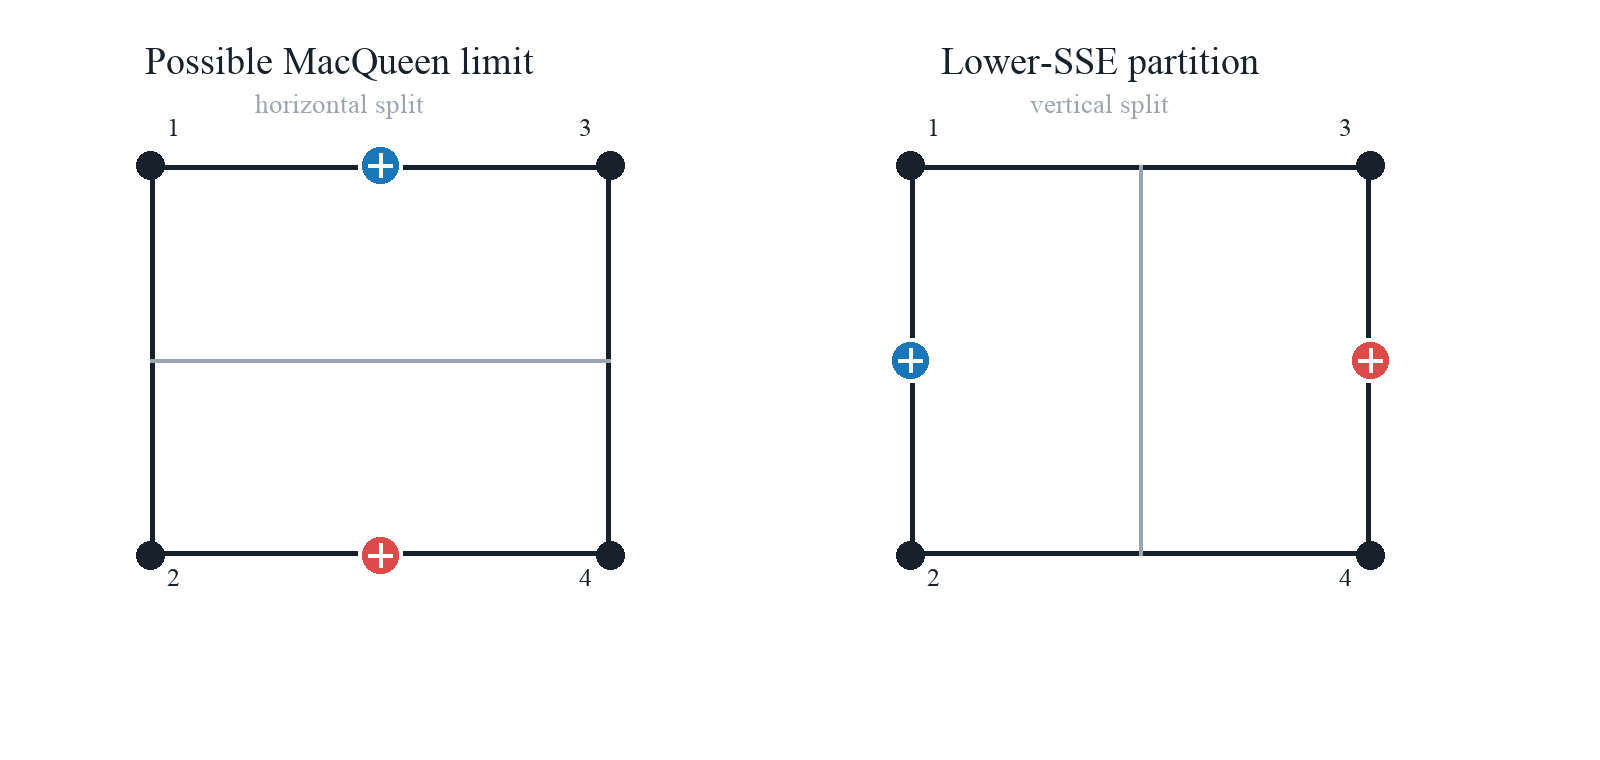
\includegraphics[width=.92\textwidth]{Figures/macqueen_rectangle.png}
    \caption{نمونه‌ی مستطیل در مقاله‌ی مک‌کوئین؛ یک حد ممکن در سمت چپ و افراز
        کم‌هزینه‌تر در سمت راست.}
    \label{fig:macqueen-rectangle}
\end{figure}

\subsection{نسخه‌ی دسته‌ای و تغییر تعداد مراکز}

بخش ۳٫۶ مقاله یک روش دسته‌ای را توصیف می‌کند: از یک افراز آغاز می‌شود،
میانگین همه‌ی خوشه‌ها هم‌زمان محاسبه می‌شود، تمام نقاط دوباره به نزدیک‌ترین
میانگین نسبت داده می‌شوند و این دو گام تکرار می‌شوند. برخلاف نسخه‌ی برخط،
در اینجا کل مجموعه‌داده در هر دور بازبینی می‌شود. روی داده‌ی متناهی، واریانس
درون‌خوشه‌ای کاهش می‌یابد و فرایند پس از تعداد متناهی گام متوقف می‌شود.

مک‌کوئین همچنین دو آستانه‌ی $C$ و $R$ را برای تغییر  تعداد مراکز
پیشنهاد می‌کند: دو مرکز با فاصله‌ی کمتر از $C$ ادغام
می‌شوند و نقطه‌ای با فاصله‌ی بیش از $R$ از نزدیک‌ترین مرکز، خود به مرکز
جدید تبدیل می‌شود.

\section{لوید و کوانتیزاسیون کمترین مربعات}

مقاله‌ی لوید
\cite{lloyd1982} ابتدا در سال ۱۹۵۷ در آزمایشگاه بل نوشته شد و در سال
۱۹۸۲ انتشار یافت. هدف، نمایش نمونه‌های ولتاژ با تعداد محدودی مقدار
بازسازی‌شده و کمینه کردنِ متوسطِ نویز کوانتیزاسیون بود.

\begin{table}[H]
    \centering
    \caption{ترجمه‌ی اصطلاحات لوید به زبان خوشه‌بندی}
    \begin{tabular}{p{.38\textwidth}p{.48\textwidth}}
        \toprule
        لوید                                & \lr{k-means}                           \\
        \midrule
        نمونه‌های ولتاژ                      & نقاط داده                              \\
        بازه‌ها یا زیرمجموعه‌های کوانتیزاسیون & خوشه‌ها                                 \\
        مقادیر کوانتیزه $q_a$               & مراکز یا میانگین‌های خوشه               \\
        نویز کوانتیزاسیون                   & مجموع مربعات خطا                   \\
        کمینه کردن متوسط نویز          & کمینه کردن فاصله‌ی مربع‌شده‌ی مورد انتظار \\
        \bottomrule
    \end{tabular}
\end{table}

\section{خروجی تعاملی فصل}

فایل \lr{interactive/macqueen-vs-lloyd.html} دو روش را روی یک داده‌ی مشترک
کنار هم نمایش می‌دهد. در سمت مک‌کوئین، هر گام فقط یک نقطه و یک میانگین را تغییر می‌دهد؛ در سمت لوید، انتساب برای همه‌ی نقاط صورت گرفته و سپس همه‌ی مراکز
به‌صورت دسته‌ای به‌روز می‌شوند.
\chapter{بهبودهای کلاسیک و انتخاب مرکز}

% \section{الگوریتم هارتیگان--وونگ}

% روش هارتیگان--وونگ \cite{hartigan1979} برخلاف لوید فقط به دنبال پایداری
% نسبت به انتساب هم‌زمان نزدیک‌ترین مرکز نیست؛ پس از مقداردهی اولیه، انتقال
% تک‌نقطه‌ای میان خوشه‌ها را مستقیماً از نظر کاهش مجموع مربعات درون‌خوشه‌ای
% می‌سنجد. برای نقطه‌ی $x$ در خوشه‌ی مبدأ $L_1$ با اندازه‌ی $n_1$، هزینه‌ی
% حذف آن متناسب با
% \begin{equation}
% \frac{n_1}{n_1-1}\lVert x-\mu_{L_1}\rVert^2
% \end{equation}
% است و افزودن آن به خوشه‌ی مقصد $L$ با اندازه‌ی $n_L$ هزینه‌ی
% \begin{equation}
% \frac{n_L}{n_L+1}\lVert x-\mu_L\rVert^2
% \end{equation}
% دارد. انتقال زمانی انجام می‌شود که کاهش خالص مثبت باشد. نقطه‌ای که تنها
% عضو خوشه‌ی خود است منتقل نمی‌شود تا خوشه‌ی تهی ایجاد نشود.

% پیاده‌سازی مرجع دو مرحله را متناوب می‌کند:
% \begin{enumerate}
% \item در \lr{OPTRA}، مقصدهای ممکن برای یک نقطه بررسی و انتقال بهبوددهنده
% انجام می‌شود. مفهوم «مجموعه‌ی زنده» از بررسی دوباره‌ی خوشه‌هایی که از آخرین
% تغییرشان ثابت مانده‌اند جلوگیری می‌کند.
% \item در \lr{QTRAN}، فقط بهترین مقصد جایگزینِ ذخیره‌شده برای هر نقطه سریع
% بررسی می‌شود. اگر انتقال انجام شود، مراکز و اندازه‌ها بلافاصله اصلاح می‌شوند.
% \end{enumerate}
% فرایند با نبود انتقال بهبوددهنده خاتمه می‌یابد. در نتیجه، جواب نسبت به
% انتقال یک نقطه یک بهینه‌ی محلی قوی‌تر است، اما همچنان تضمین بهینه‌ی سراسری
% ندارد. فایل \lr{interactive/hartigan-wong-vs-lloyd.html} تفاوت انتقال‌های
% تک‌نقطه‌ای با دورهای دسته‌ای لوید را به‌صورت مفهومی و گام‌به‌گام نمایش می‌دهد.

\section{مقداردهی اولیه‌ی \lr{k-means++}}

آرتور و واسیلیویتسکی نشان دادند که انتخاب دقیق‌تر مراکز اولیه می‌تواند
کیفیت مورد انتظار \lr{k-means} را کنترل کند \cite{arthur2007}. الگوریتم
\lr{k-means++} چنین است:
\begin{enumerate}
    \item مرکز نخست به‌صورت یکنواخت از نقاط داده انتخاب می‌شود.
    \item اگر $D(x)$ فاصله‌ی نقطه‌ی $x$ تا نزدیک‌ترین مرکز انتخاب‌شده باشد،
          مرکز بعدی با احتمال
          \begin{equation}
              P(x)=
              \frac{D(x)^2}{\sum_{x'\in\mathcal{X}}D(x')^2}
          \end{equation}
          انتخاب می‌شود.
    \item گام دوم تا انتخاب $k$ مرکز تکرار و سپس الگوریتم معمول لوید اجرا می‌شود.
\end{enumerate}
این نمونه‌گیری «وزن‌دهی $D^2$» نام دارد. قضیه‌ی اصلی مقاله بیان می‌کند
\begin{equation}
    \mathbb{E}[\Phi]\leq 8(\ln k+2)\Phi_{\mathrm{OPT}}.
    \label{eq:kpp-bound}
\end{equation}
بنابراین روش در بدترین حالت
$O(\log k)$-رقابتی است و برای نمونه‌های خوب می‌تواند کران ثابت
داشته باشد. روش پیشینِ استروفسکی و همکاران، کران ثابت را تحت شرط
\begin{equation}
    \frac{\Phi_{\mathrm{OPT},k}}
    {\Phi_{\mathrm{OPT},k-1}}\leq\varepsilon^2
\end{equation}
به دست می‌داد؛ یعنی جواب $k$-خوشه‌ای باید به‌طور محسوسی بهتر از جواب
$(k-1)$-خوشه‌ای باشد.

\begin{lemma}[هویت مرکز ثقل]
    برای مجموعه‌ی متناهی $S$، مرکز ثقل $c(S)$ و هر نقطه‌ی $z$ داریم
    \begin{equation}
        \sum_{x\in S}\lVert x-z\rVert^2
        =
        \sum_{x\in S}\lVert x-c(S)\rVert^2
        +|S|\lVert c(S)-z\rVert^2.
        \label{eq:centroid-identity}
    \end{equation}
\end{lemma}

تفسیر رابطه‌ی \ref{eq:centroid-identity} این است که هزینه‌ی انتخاب هر
نماینده‌ی دلخواه برابر است با هزینه‌ی (فاصله‌ی) نقاط نسبت به مرکز ثقل واقعی،
به‌علاوه‌ی جریمه‌ی دور بودن آن نماینده از مرکز ثقل که در تعداد نقاط ضرب
می‌شود. 
\section{سایر مسیرهای مطالعه‌شده}

\subsection{روش \lr{global k-means}}

روش \lr{global k-means} \cite{likas2003} مراکز را یکی‌یکی اضافه می‌کند. برای
افزایش تعداد خوشه‌ها از $k-1$ به $k$، هر نقطه‌ی داده یک‌بار به‌عنوان مرکز
جدید در کنار جواب قبلی آزمایش و لوید اجرا می‌شود؛ بهترین جواب نگه داشته
می‌شود. این جست‌وجوی قطعی حساسیت به مقداردهی اولیه را کاهش می‌دهد، اما
اجرای مکرر آن پرهزینه است. نسخه‌ی سریع مقاله با یک کران کاهش خطا، نامزدها
را محدود می‌کند.

\subsection{\lr{X-means}}

\lr{X-means} \cite{pelleg2000} از یک کران پایین برای $k$ آغاز می‌کند و
خوشه‌ها را به‌صورت محلی برای شکستن به دو بخش نامزد می‌کند. این فرایند تا کران بالای $k$ ادامه
می‌یابد. مزیت اصلی آن جست‌وجوی هم‌زمان ساختار و تعداد خوشه‌هاست، ولی نتیجه
به مدل آماری و بازه‌ی مجاز $k$ وابسته است.

\chapter{الگوریتم \lr{GLKM}}

\section{انگیزه و بازنویسی تابع هدف}

مقاله‌ی اصلی پروژه، \lr{GLKM}، روشی حریصانه برای بهینه‌سازی
\lr{k-means} ارائه می‌کند \cite{yuan2026}. زوجی بودن تابع جریمه
\begin{equation}
    \sum_{x\in S}\lVert x-\mu_S\rVert^2
    =
    \frac{1}{2|S|}
    \sum_{x,y\in S}\lVert x-y\rVert^2
    \label{eq:pairwise}
\end{equation}
اجازه می‌دهد هزینه‌ی هر خوشه بدون نمایش صریح مرکز آن و با استفاده از
فاصله‌های زوجی محاسبه شود. \lr{GLKM} از $n$ خوشه‌ی تک‌عضوی شروع می‌کند و در
هر مرحله زوجی را ادغام می‌کند که کمترین افزایش تابع هدف را داشته باشد؛ این
روند تا رسیدن به تعداد خوشه‌ی درخواستی $k$ ادامه می‌یابد.

\section{ماتریس فاصله}

نگهداری همه‌ی $n^2$ فاصله برای داده‌ی بزرگ مناسب نیست. مقاله یک گراف
$K$-نزدیک‌ترین همسایه می‌سازد. برای یال‌های موجود، فاصله‌ی مربع‌شده‌ی واقعی
و برای زوج‌های فاقد یال مقدار  $\gamma$ در نظر گرفته می‌شود؛
$\gamma$ بر مبنای بزرگ‌ترین فاصله‌ی موجود در گراف تنظیم می‌شود. در نتیجه،
هدف محاسبه‌شده دقیقاً تابع هدف اقلیدسی کامل نیست، بلکه تقریب آن
است. 

\section{شتاب‌دهی‌ها}

سه ایده‌ی اصلی برای کاهش هزینه‌ی جست‌وجوی ادغام‌ها به‌کار رفته است:
\begin{enumerate}
    \item به‌روزرسانی جبری هزینه‌ی ادغام با نگهداری آمار خوشه‌ها، به‌جای
          محاسبه‌ی دوباره‌ی تمام فاصله‌ها؛
    \item محدود کردن زوج‌های نامزد به همسایگی گراف:؛
    \item نگهداری نامزدهای ادغام در ساختاری مرتب برای دسترسی سریع به کمترین
          افزایش.
\end{enumerate}

\section{ایده‌ها برای توسعه این پروژه}

دو پرسش از مطالعه‌ی روش حاصل شد:
\begin{enumerate}
    \item آیا می‌توان با اجرای \lr{GLKM} روی چند مقدار $k$ و نمودار elbow
          نیاز به دریافت $k$ از کاربر را ااز بین برد؟
    \item آیا می‌توان به‌جای آغاز از $n$ خوشه‌ی تک‌عضوی، یک افراز اولیه‌ی کوچک‌تر
          ساخت تا تعداد ادغام‌ها و زمان اجرای هسته‌ی \lr{GLKM} کاهش یابد؟
\end{enumerate}
فصل‌های بعدی پیاده‌سازی و ارزیابی مقدماتی این دو پرسش را گزارش می‌کنند.

\chapter{بررسی روش آرنج برای تخمین تعداد خوشه‌ها}

\section{آزمایش نخست: داده‌ی \lr{D1}}

آزمایش برای $k=2,\ldots,10$ و گراف ۱۲-نزدیک‌ترین همسایه اجرا شد و هزینه برابر
$100936.0647$ باقی ماند. در نتیجه هیچ منحنی آرنج معناداری ساخته نشد.

\section{آزمایش دوم: داده‌ی \lr{Gisette}}

برای داده‌ی \lr{Gisette} با گراف ۸۰-نزدیک‌ترین همسایه، الگوریتم به همه‌ی
مقادیر درخواستی رسید. نتایج تابع هدف در جدول \ref{tab:gisette-elbow} آمده است.

\begin{table}[H]
\centering
\caption{هزینه‌ی \lr{GLKM} روی \lr{Gisette} برای مقادیر مختلف $k$}
\label{tab:gisette-elbow}
\begin{tabular}{cccccccccc}
\toprule
$k$ & 2 & 3 & 4 & 5 & 6 & 7 & 8 & 9 & 10\\
\midrule
$\Phi/10^7$ & \lr{2.586} & \lr{2.580} & \lr{2.574} & \lr{2.568} & \lr{2.563} & \lr{2.557} & \lr{2.552} & \lr{2.546} & \lr{2.541}\\
\bottomrule
\end{tabular}
\end{table}

روش فاصله از وتر $k=5$ را انتخاب کرد؛ بااین‌حال کاهش هزینه تقریباً خطی است. همچنین معیارهای \lr{ACC} و \lr{NMI} در
$k=2$ بهتر بودند. بنابراین $k=5$ بیشتر محصول حساسیت هندسی روش eblow
است.

\begin{figure}[H]
\centering
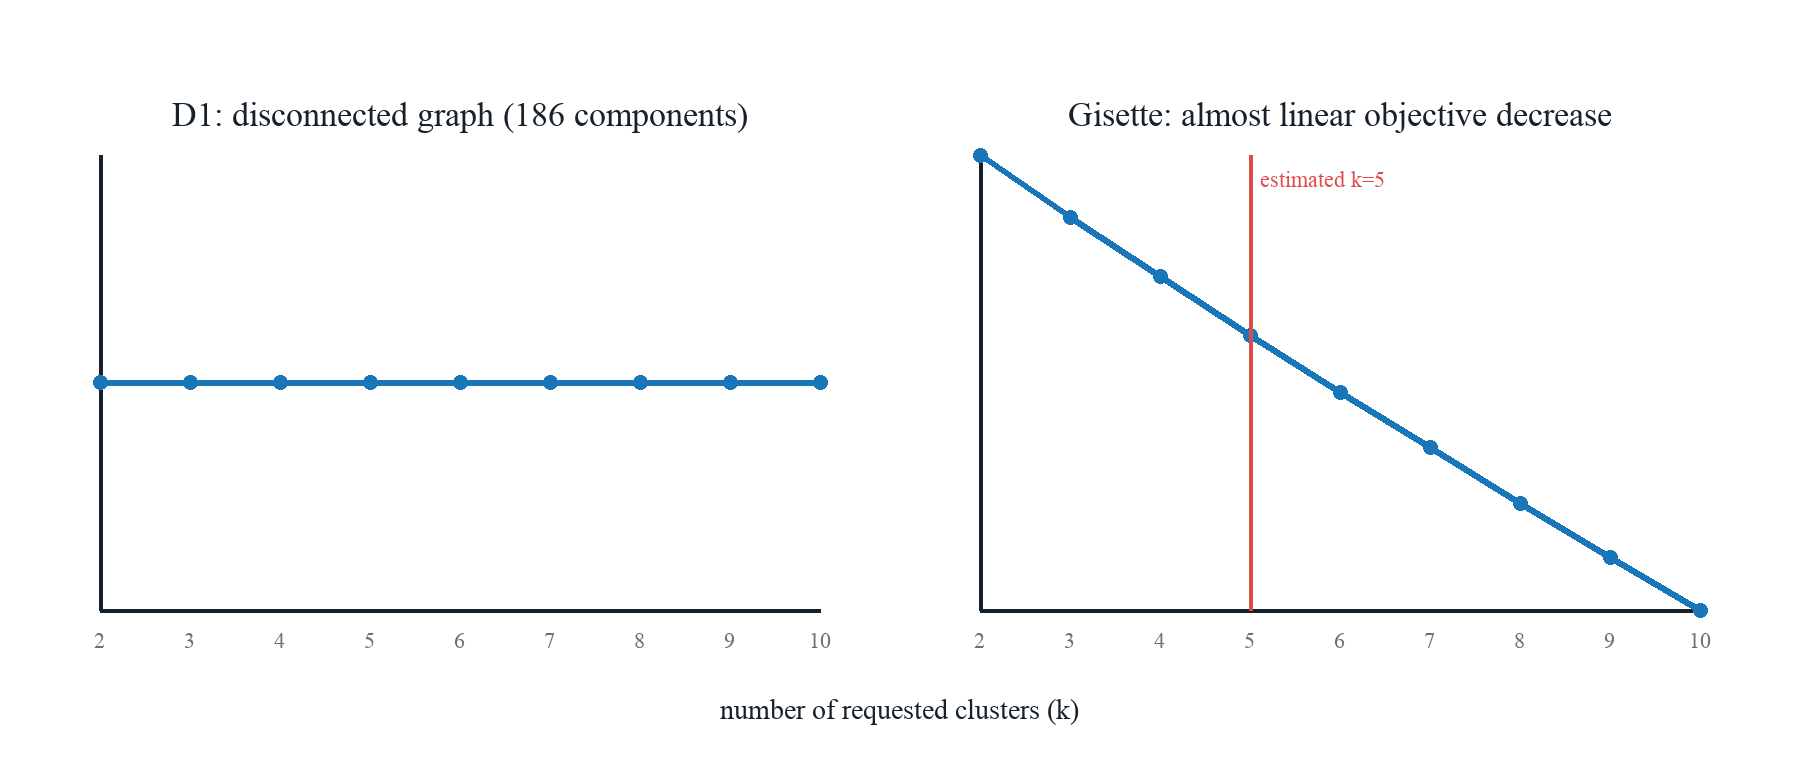
\includegraphics[width=\textwidth]{Figures/elbow_results.png}
\caption{دو شکست روش آرنج}
\label{fig:elbow-results}
\end{figure}

\section{جمع‌بندی آزمایش}

روش آرنج در شکل فعلی جایگزین مطمئنی برای ورودی $k$ نیست.هرچند بر اساس یافته‌های فعلی می‌توان در آینده مسیر توسعه بهتری را در پیش گرفت.


\chapter{افراز اولیه‌ی \lr{k-means++} برای \lr{GLKM}}

\section{صورت دقیق ایده}

در نسخه‌ی اصلی \lr{GLKM} هر نقطه یک خوشه‌ی تک‌عضوی است؛ بنابراین برای رسیدن
به $k$ خوشه تقریباً $n-k$ ادغام لازم است. ایده‌ی آزمایش‌شده آن بود که ابتدا
$m=\alpha k$ خوشه بسازیم و سپس \lr{GLKM} را از این افراز آغاز کنیم تا فقط
$m-k$ ادغام انجام شود.

\section{نتایج مقدماتی روی \lr{Gisette}}

آزمایش نخست با $k=2$ و گراف ۸۰-نزدیک‌ترین همسایه انجام شد. جدول \ref{tab:kpp-fast} زمان کل و
معیارهای بیرونی را نشان می‌دهد.

\begin{table}[H]
    \centering
    \caption{اثر اندازه‌ی افراز اولیه؛ عبارت $10k$ یعنی آغاز از ۲۰ خوشه}
    \label{tab:kpp-fast}
    \begin{tabular}{lrrrr}
        \toprule
        آغاز          & زمان کل (ثانیه) & هزینه‌ی تقریبی ($10^7$) & \lr{ACC}   & \lr{NMI}   \\
        \midrule
        تک‌عضوی (اصلی) & \lr{1.33}       & \lr{2.586}             & \lr{0.795} & \lr{0.358} \\
        $4k$          & \lr{2.78}       & \lr{2.562}             & \lr{0.577} & \lr{0.033} \\
        $10k$         & \lr{3.28}       & \lr{2.561}             & \lr{0.748} & \lr{0.210} \\
        $25k$         & \lr{3.73}       & \lr{2.561}             & \lr{0.588} & \lr{0.054} \\
        $100k$        & \lr{10.87}      & \lr{2.563}             & \lr{0.760} & \lr{0.269} \\
        \bottomrule
    \end{tabular}
\end{table}

\begin{figure}[H]
    \centering
    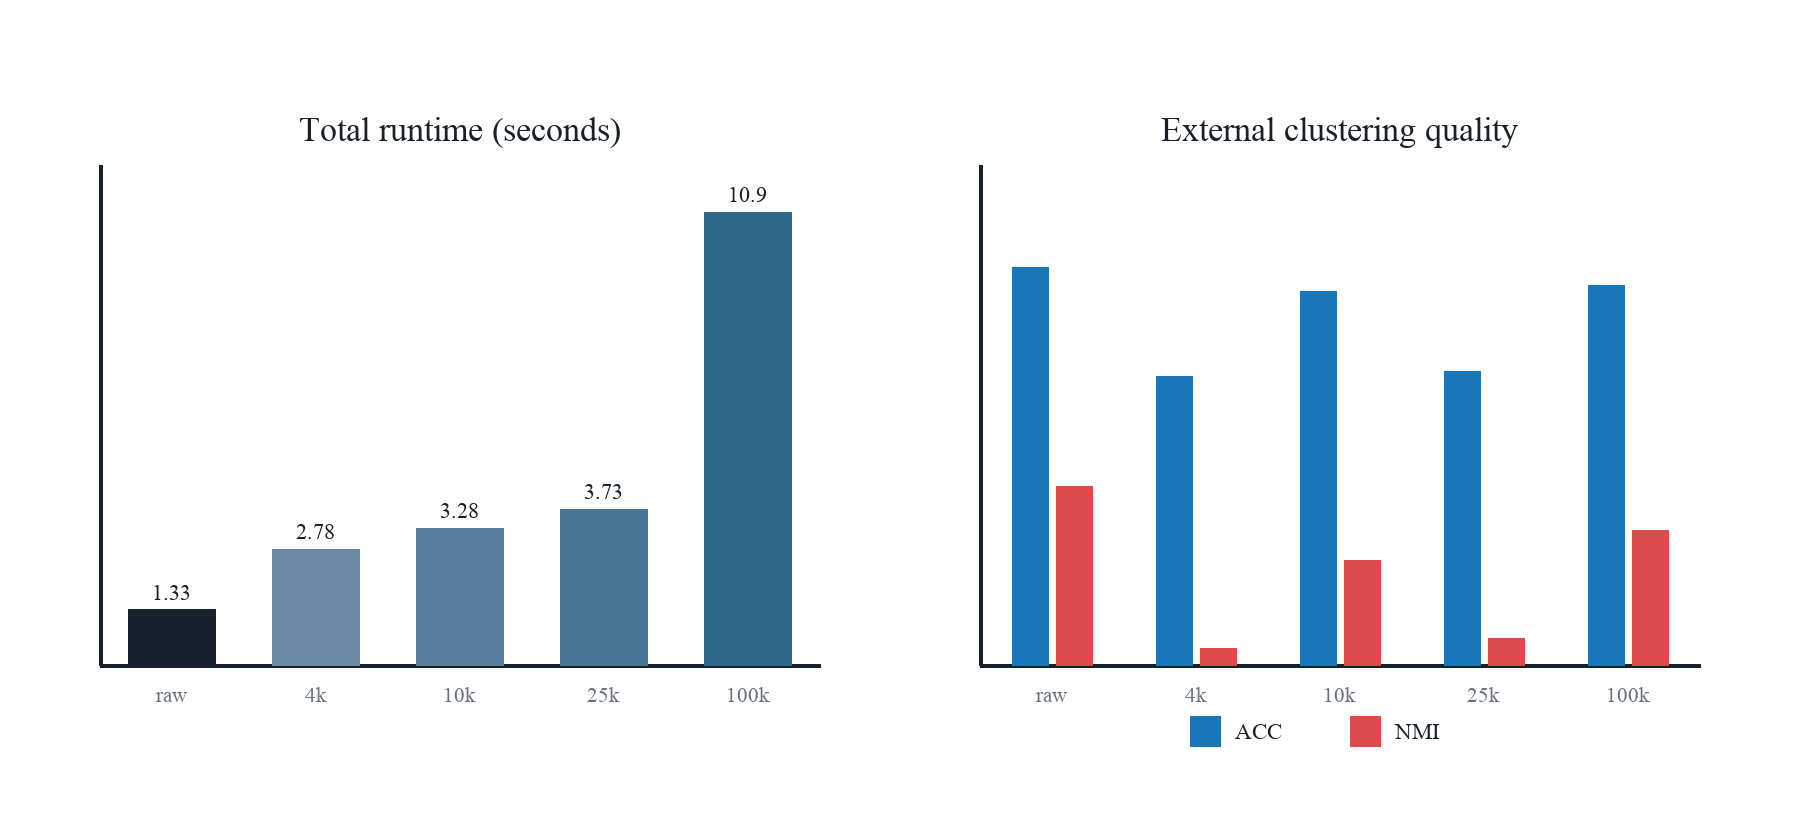
\includegraphics[width=\textwidth]{Figures/kpp_results.png}
    \caption{زمان کل و کیفیت برای افرازهای اولیه‌ی مختلف روی
        \lr{Gisette}.}
    \label{fig:kpp-results}
\end{figure}

افراز اولیه تعداد ادغام‌های هسته را کاهش می‌دهد، اما هزینه‌ی اجرای
\lr{KMeans} مقدماتی باعث شد زمان کل در همه‌ی حالت‌ها از روش اصلی بیشتر
شود. هزینه‌ی تقریبی داخلی کمی کاهش یافت، ولی \lr{ACC} و \lr{NMI} بدتر

\section{نتیجه‌گیری کلی}

دستاورد این مرحله بیش از آن‌که یک الگوریتم بهتر باشد، تبدیل دو ایده‌ی اولیه
به فرضیه‌های قابل‌آزمون و مشخص کردن حالت‌های شکست آن‌هاست. روش elbow قابل اتکا نیست. افراز اولیه‌ی فعلی نیز در آزمایش
انجام‌شده زمان کل و کیفیت بیرونی را بهبود نداد. در مقابل، مطالعه‌ی منابع
تاریخی و جدید، ایجاد ابزارهای تکرارپذیر، بهبود زمان و ساخت صفحات
تعاملی، پایه‌ی روشنی برای مرحله‌ی بعد پروژه فراهم کرده است.



%
%\phantomsection\addcontentsline{toc}{chapter}{منابع و مآخذ}
%\nocite{*}
%
%\small
%\bibliographystyle{IEEEtran}
%%\bibliographystyle{chicago-fa}  %Similar to the apacite style
%\bibliography{References.bib} % Your BibTeX file
\renewcommand{\bibname}{منابع و مآخذ}
\small
\begin{thebibliography}{99}

\bibitem{macqueen1967}
\lr{J. MacQueen, ``Some Methods for Classification and Analysis of
Multivariate Observations,'' in Proceedings of the Fifth Berkeley Symposium
on Mathematical Statistics and Probability, vol. 1, pp. 281--297, 1967.}

\bibitem{lloyd1982}
\lr{S. P. Lloyd, ``Least Squares Quantization in PCM,'' IEEE Transactions
on Information Theory, vol. 28, no. 2, pp. 129--137, 1982.}

\bibitem{hartigan1979}
\lr{J. A. Hartigan and M. A. Wong, ``Algorithm AS 136: A K-Means
Clustering Algorithm,'' Journal of the Royal Statistical Society, Series C
(Applied Statistics), vol. 28, no. 1, pp. 100--108, 1979.}

\bibitem{arthur2007}
\lr{D. Arthur and S. Vassilvitskii, ``k-means++: The Advantages of Careful
Seeding,'' in Proceedings of the 18th Annual ACM-SIAM Symposium on Discrete
Algorithms (SODA), pp. 1027--1035, 2007.}

\bibitem{likas2003}
\lr{A. Likas, N. Vlassis, and J. J. Verbeek, ``The Global k-means
Clustering Algorithm,'' Pattern Recognition, vol. 36, no. 2, pp. 451--461,
2003.}

\bibitem{pelleg2000}
\lr{D. Pelleg and A. Moore, ``X-means: Extending K-means with Efficient
Estimation of the Number of Clusters,'' in Proceedings of the 17th
International Conference on Machine Learning, pp. 727--734, 2000.}

\bibitem{frahling2008}
\lr{G. Frahling and C. Sohler, ``A Fast k-Means Implementation Using
Coresets,'' International Journal of Computational Geometry \&
Applications, vol. 18, no. 6, pp. 605--625, 2008.}

\bibitem{choo2020}
\lr{D. Choo, C. Grunau, J. Portmann, and V. Rozhon, ``k-means++: Few More
Steps Yield Constant Approximation,'' in Proceedings of the 37th
International Conference on Machine Learning, pp. 1909--1917, 2020.}

\bibitem{yuan2026}
\lr{Y. Yuan, L. Zhao, S. Pei, and F. Nie, ``Efficient Greedy Optimization
Method for k-means,'' Pattern Recognition, vol. 171, p. 112140, 2026.}

\end{thebibliography}


\end{document}
